\begin{tikzpicture}[font=\footnotesize]
\node (A) at (0,0) [minimum size=1cm] {}; \Alice{0}{0}{0.4};
\node (B) [right of = A, node distance = 4cm, minimum size=1cm] {}; \Bob{4cm}{0}{0.4};
\node (0a1) [below of=A, node distance=0.7cm] {$b \gets \{H,T\}$};
\node (0b1) [below of=B, node distance=0.7cm] {};
\node (1a) [below of=0a1, node distance=0.5cm] {$m = b\| r$, $r$ is random};
\node (1b) [below of=0b1, node distance=0.5cm] {};
\node (2a) [below of=1a, node distance=0.5cm] {$h = \mathsf{Hash}(m)$};
\node (2b) [below of=1b, node distance=0.5cm] {};
\draw[-latex] (2a) -- (2b) node [midway,above] {};
\node (3a) [below of=2a, node distance=0.5cm] {};
\node (3b) [below of=2b, node distance=0.5cm] {$b' \in \{H,T\}$};
\draw[-latex] (3b) -- (3a) node [midway,above] {};
\node (4a) [below of=3a, node distance=0.5cm] {$m$};
\node (4b) [below of=3b, node distance=0.5cm] {$h \overset{?}{=} \mathsf{Hash}(m)$};
\draw[-latex] (4a) -- (4b) node [midway,above] {};
\node (5a) [below of=4a, node distance=0.5cm] {};
\node (5b) [below of=4b, node distance=0.5cm] {};
\node (6b) [below of=4b, node distance=0.5cm] {Win if $b=b'$};
\end{tikzpicture}
